% !TEX root = ../Diplombericht.tex
\section{Konzept} 
\label{sec:Konzept}
Das Konzept beschreibt den vorgesehenen Aufbau des Clusters und beinhaltet die Testfälle welche bei der Abnahme nach der Realisierung berücksichtigt werden müssen.

\subsection{Aufbau}
Die Infrastruktur des Clusters soll wie folgt aussehen:

\begin{figure}[htb]
\centering
\includegraphics[scale=0.6]{Systemlandschaft.jpg}
\caption{Systemlandschaft}
\label{fig:Systemlandschaft}
\end{figure} 

\textbf{Benötigte Protokolle}
\begin{table}[H]
\centering
\begin{tabular}{p{1cm}p{5cm}p{5cm}p{5cm}}
\hline
\rowcolor{heading} \textbf{Nr.} & \textbf{Protokoll} & \textbf{Protokollfamilie} & Ports \\\hline
1 & SSH & TCP & 22 \\\hline
2 & SMB & TCP & 445 \\\hline
3 & DHCP & UDP & 67 / 78 \\\hline
4 & TFTP & UDP & 69 \\\hline
5 & HTTP & TCP & 80 \\\hline
\end{tabular}
\caption{Protokolle}
\end{table}
\subsubsection{Physikalische Verbindungen}

\textbf{Stromversorgung Managementnode}\newline
Der Managementnode wird über den Micro USB Anschluss mit Strom versorgt. Dabei muss darauf geachtet werden, dass ein mindest Strom von 2 Ampere und ein maximaler Strom von 2.5 Ampere fliesst. Zudem wird eine konstante Spannung von 5 Volt benötigt. Deshalb wird ein Netzteil mit einer Leistung von 12.5 Watt benötigt. Das Netzteil wird über eine Stromschiene an das Stromnetz angeschlossen.

\textbf{Stromversorgung Computenodes}\newline
Die Managementnodes werden über die GPIO Pins 2 und 6 mit Strom versorgt (siehe Abbildung ). Dazu werden Jumper Kabel benötigt. Da es sich hierbei um eine Anzahl von mindestens 40 Raspberry's handelt ist ein Netzteil mit einer Leistung von 500W vorgesehen. Das Netzteil wird über die Stromschiene an das Stomnetz angeschlossen.

\begin{figure}[htb]
\centering
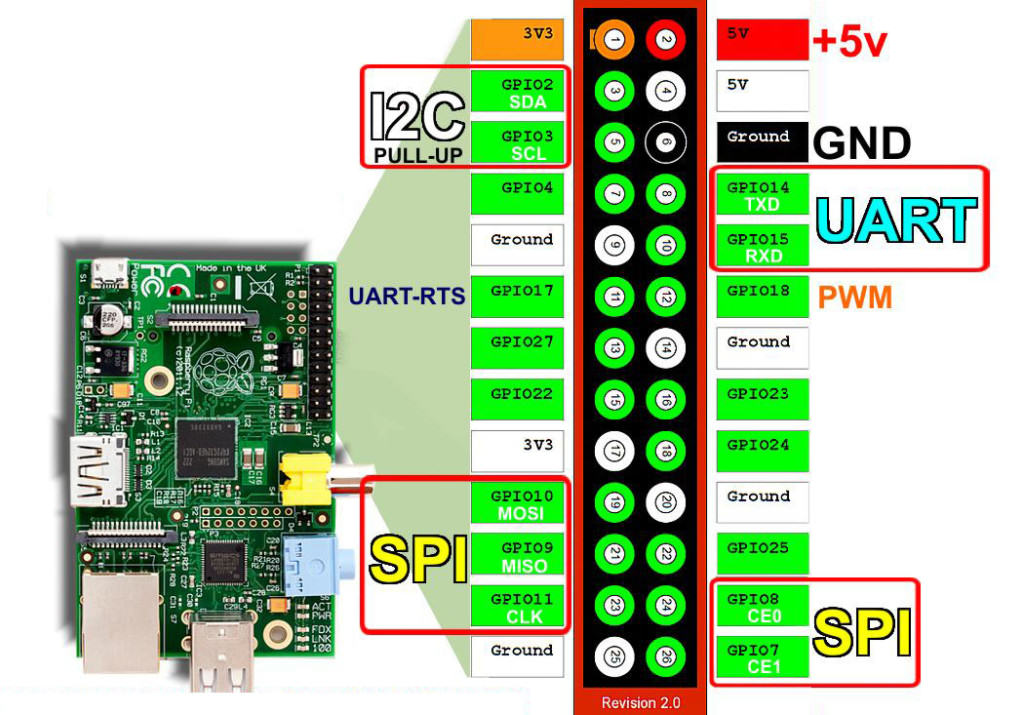
\includegraphics[scale=0.5]{rpi_gpio.jpg}
\caption{GPIO Anschlüsse}
\label{fig:GPIO Anschlüsse}
\end{figure} 

Quelle: https://developer-blog.net/wp-content/uploads/2013/09/raspberry-pi-rev2-gpio-pinout-1024x715.jpg

\textbf{Stromversorgung übriger Geräte}\newline
Die übrigen Geräte werdenüber den herkömmlichen Weg mit Strom über eine Stromschiene versorgt.

\textbf{Netzwerkverbindungen}\newline
Die folgenden Komponenten sind über den Switch in das lokale Netzwerk eingebunden, die nicht aufgelisteten Geräte werden direkt über Powerline oder WLAN mit dem Router verbunden.
\begin{itemize}
\item Managementnode
\item Computenodes
\item NAS
\end{itemize}

\subsubsection{Technische Verbindungen \& Kommunikation}
\begin{table}[H]
\centering
\begin{tabular}{p{1cm}p{1.5cm}p{1.5cm}p{2.2cm}p{9.8cm}}
\hline
\rowcolor{heading} \textbf{Nr.} & \textbf{Quelle} & \textbf{Ziel }& \textbf{Betrifft} & \textbf{Beschreibung} \\\hline
1 & NAS & Mgmt & Datenablage & Der NAS Share wird über das SMB Protkoll angehängt. \\\hline
2 & NAS & Compute & Datenablage & Der NAS Share wird über das SMB Protkoll angehängt. \\\hline
3 & Router & Mgmt & IP Adresse & Anhand der MAC Adresse wird eine statische IP Adresse zugewiesen. \\\hline
4 & Router & Compute & IP Adressen & Anhand der MAC Adressen werden statische IP Adressen zugewiesen. \\\hline
5 & Router & Mgmt &Hostname & Es wird über den Router ein definierter Hostname verteilt. \\\hline
6 & Router & Compute & Hostnamen & Es werden über den Router definierte Hostnamen verteilt. \\\hline
7 & Mgmt & Compute & Netzwerkboot & Der Managementnode beliefert die Computenodes über das TFT Protkoll mit dem Betriebssystem \\\hline
8 & Internet & Mgmt & Zeitserver & Die aktuelle Zeit wird mit NTP über das Internet synchronisiert.\\\hline
8 & Mgmt & Compute & Zeitserver & Die Computenodes beziehen die aktuelle Zeit über NTP.\\\hline
9 & Internet & Compute & Internetzugriff & Die Computenodes können über ein routing über den Mgmt auf das Internet zugreifen. \\\hline
10 & PC & Mgmt & Zugriff & Verbindungen über den PC können mit dem SSH Protokoll aufgebaut werden. \\\hline
11 & PC & Compute & Zugriff & Verbindungen über den PC können mit dem SSH Protokoll aufgebaut werden. \\\hline
\end{tabular}
\caption{Verbindungen \& Kommunikation}
\end{table}
\textbf{Legende:} Mgmt = Managementnode, Compute = Computenode, PC = Home Computer

\newpage
\subsection{Hostnamen}
Die Computenamen wurden nach einem überschaulichen Konzept definiert. Jeder Computenode trägt den Prefix "c". Dies soll bei der Behebung von Problemen auf physicher Ebene, z.B. Austauschen eines Nodes dienen. Zudem werden alle Hostnamen immer in kleinen Buchstaben geschrieben.

\subsubsection{Managementnode Name}
\begin{table}[H]
\centering
\begin{tabular}{p{5cm}p{5.5cm}p{5.5cm}}
\hline
\rowcolor{heading} \textbf{Name} & \textbf{IP} & \textbf{MAC} \\\hline
nebula & 192.168.1.10 & B8:27:EB:32:A9:1C \\\hline
\end{tabular}
\caption{Managementnode Name}
\end{table}

\subsubsection{Reservenode Name}
Die Reservenodes sind als Fallback für ausgefallene Computenodes vorgesehen.
\begin{table}[H]
\centering
\begin{tabular}{p{1cm}p{2cm}p{6cm}p{6cm}}
\hline
\rowcolor{heading} \textbf{Nr.} & \textbf{Name} & \textbf{IP} & \textbf{MAC} \\\hline
1 & c36 & 192.168.1.51 & x\\\hline
2 & c37 & 192.168.1.52 & x\\\hline
3 & c38 & 192.168.1.53 & x\\\hline
4 & c39 & 192.168.1.54 & x\\\hline
5 & c40 & 192.168.1.55 & x\\\hline
\end{tabular}
\caption{Reservenode Name}
\end{table}

\subsubsection{Computenode Namen}
\begin{table}[H]
\centering
\begin{tabular}{p{1cm}p{2cm}p{6cm}p{6cm}}
\hline
\rowcolor{heading} \textbf{Nr.} & \textbf{Name} & \textbf{IP} & \textbf{MAC} \\\hline
1 & c1 & 192.168.1.11 & B8:27:EB:32:39:A7\\\hline
2 & c2 & 192.168.1.12 & B8:27:EB:2E:A3:D1\\\hline
3 & c3 & 192.168.1.13 & B8:27:EB:50:45:3F\\\hline
4 & c4 & 192.168.1.14 & B8:27:EB:0D:E6:25\\\hline
5 & c5 & 192.168.1.15 & B8:27:EB:3E:96:B5\\\hline
6 & c6 & 192.168.1.16 & B8:27:EB:EE:77:DA\\\hline
7 & c7 & 192.168.1.17 & B8:27:EB:21:63:E6\\\hline
8 & c8 & 192.168.1.18 & B8:27:EB:2E:2E:CC\\\hline
9 & c9 & 192.168.1.19 & B8:27:EB:17:32:96\\\hline
10 & c10 & 192.168.1.20 & B8:27:EB:B2:1C:A9\\\hline
11 & c11 & 192.168.1.21 & B8:27:EB:AF:63:1F\\\hline
12 & c12 & 192.168.1.22 & B8:27:EB:43:00:2C\\\hline
13 & c13 & 192.168.1.23 & B8:27:EB:13:7B:18\\\hline
14 & c14 & 192.168.1.24 & B8:27:EB:43:CD:29\\\hline
15 & c15 & 192.168.1.25 & B8:27:EB:FF:C7:56\\\hline
16 & c16 & 192.168.1.26 & B8:27:EB:CE:98:66\\\hline
17 & c17 & 192.168.1.27 & B8:27:EB:5D:63:34\\\hline
18 & c18 & 192.168.1.28 & B8:27:EB:91:3E:0F\\\hline
19 & c19 & 192.168.1.29 & B8:27:EB:F4:65:EC\\\hline
20 & c20 & 192.168.1.30 & B8:27:EB:3E:AB:DC\\\hline
21 & c21 & 192.168.1.31 & B8:27:EB:66:60:F6\\\hline
22 & c22 & 192.168.1.32 & B8:27:EB:37:3F:74\\\hline
23 & c23 & 192.168.1.33 & B8:27:EB:18:5E:F0\\\hline
24 & c24 & 192.168.1.34 & B8:27:EB:B0:23:B8\\\hline
25 & c25 & 192.168.1.35 & B8:27:EB:BE:C4:94\\\hline
26 & c26 & 192.168.1.36 & B8:27:EB:FB:FF:57\\\hline
27 & c27 & 192.168.1.37 & B8:27:EB:4E:EC:CE\\\hline
28 & c28 & 192.168.1.38 & B8:27:EB:43:1C:35\\\hline
29 & c29 & 192.168.1.39 & B8:27:EB:DC:74:5F\\\hline
30 & c30 & 192.168.1.40 & B8:27:EB:D1:DE:2F\\\hline
31 & c31 & 192.168.1.41 & B8:27:EB:5E:90:34\\\hline
32 & c32 & 192.168.1.42 & B8:27:EB:DE:80:24\\\hline
33 & c33 & 192.168.1.43 & B8:27:EB:A4:79:6F\\\hline
34 & c34 & 192.168.1.44 & B8:27:EB:0A:4D:C7\\\hline
35 & c35 & 192.168.1.45 & B8:27:EB:5C:53:5F\\\hline
36 & c36 & 192.168.1.46 & B8:27:EB:F7:AF:C2\\\hline
37 & c37 & 192.168.1.47 & B8:27:EB:CE:BA:ED\\\hline
38 & c38 & 192.168.1.48 & B8:27:EB:59:38:3C\\\hline
39 & c39 & 192.168.1.49 & B8:27:EB:99:BB:8E\\\hline
40 & c40 & 192.168.1.50 & B8:27:EB:8F:7A:0D\\\hline
\end{tabular}
\caption{Computenode Namen}
\end{table}


\subsection{Design der Lösung}
\begin{itemize}
	\item Grob- und Detaildesign, Prozesse, Abläufe etc. erstellen. Alle Zusaamenhänge müssen nachvollziehbar und transparent sein!
\end{itemize}

